

%%%%%%%%%%%%%%%%%%%%%%%%%%%%
% SECTION                  %
%%%%%%%%%%%%%%%%%%%%%%%%%%%%

\textbf{Introduction} \\
Dans ce chapitre nous allons présenter en premier lieu l'entreprise d'accueil CNUDST, d’une   manière   générale, sa structure organisationnelle, ses missions et son historique.\\ En second lieu nous allons nous focaliser sur l'étude des besoins de l'utilisateur, nous allons détailler les besoins fonctionnels et les exigences non fonctionnelles de l'application.\\ En dernier lieu, nous allons traiter la dernière section qui porte sur l'étude de l'existant.
\section{Présentation de l’entreprise}
Le CNUDST est un centre intégré d’information scientifique et technique. Le CNUDST a pour missions essentielles de :
\begin{itemize}
	\item Fournir l’information et la documentation scientifique et technique notamment aux chercheurs, quel que soit leur domaine d’activité.
	\item Collecter, traiter et diffuser la production et les résultats de la recherche scientifique et du développement technologique entrepris en Tunisie ou portant sur la Tunisie.
	\item Permettre un accès convivial à un fonds documentaire couvrant une partie importante de la recherche scientifique et technologique à l’échelle mondiale.
	\item Pratiquer la veille documentaire.
\end{itemize}
Pour ce faire, des applications sous forme de bases et de banques de données ont été développées dans le but de:
\begin{itemize}
	\item Valoriser les résultats des recherches et contribuer à la promotion de la production scientifique tunisienne en assurant sa visibilité sur le web.
	\item Assurer une veille documentaire permanente sur les ressources documentaires accessibles sur le web à titre gratuit ou à tarif préférentiel (programmes en faveur des pays en développement).
	\item Mettre à la disposition des chercheurs la littérature scientifique mondiale nécessaire à leur activité, par la conclusion de licences avec des éditeurs internationaux en différentes spécialités pour l’accès à des revues en texte intégral et des bases et banques de données.
\end{itemize}
\section{Historique}
Le Centre National Universitaire de Documentation Scientifique et Technique est un établissement public à caractère administratif doté de la personnalité civile et de l’autonomie financière, relevant de la tutelle du Ministère de l’Enseignement Supérieur et de la Recherche Scientifique.
Il a été créé par la loi n° 78-59 du 29/12/1978\footnote{\url{http://cnudst.rnrt.tn/wp-content/uploads/2016/07/78-59-fr.pdf}} portant loi de finances pour la gestion 1979 et notamment son article 33, et géré par décret n° 99-2241 du 11/10/1999. 
\section{Organigramme}
\begin{figure}[!p]
	\centering
{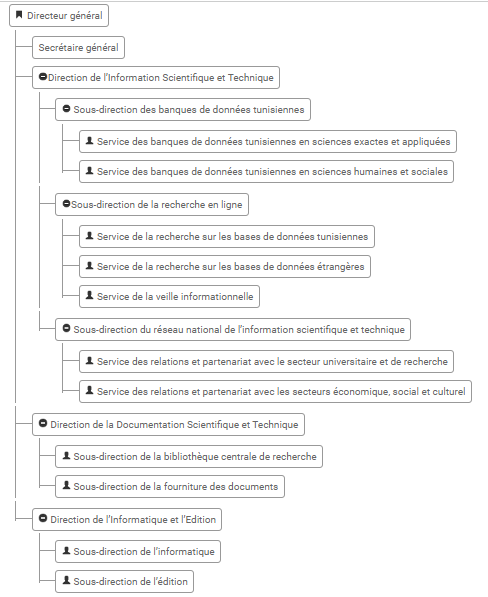
\includegraphics[width=0.95\textwidth]{D) IMAGES/imOrg.png}}
	\caption{Organigramme}
	\label{Org}
\end{figure}

Au sommet, nous trouvons la direction générale. Au deuxième niveau nous trouvons le secrétariat général, la Direction de l'information scientifique et technique, la direction de la documentation scientifique et technique et la direction de l'informatique et de l'édition. Au troisième niveau, nous trouvons les sous-directions.
\newpage
%\section{Problématique}

	

\section{Etude de l’existant } 
Pour gérer les inscriptions aux formations en ligne, le CNUDST lance un formulaire de préinscription via « Google Forms » sur son site web pendant une période bien déterminée.\\
Cependant,  après sa dernière constatation concernant la violation à grande échelle des données personnelles détectée dans le milieu universitaire tunisien, l’instance nationale de protection des données personnelles (INPDP) rappelle dans son article publié le 28 octobre 2021\footnote{\url{https://www.webmanagercenter.com/2021/10/28/474672/violation-a-grande-echelle-des-donnees\\-personnelles-dans-le-milieu-universitaire-tunisien-sinquiete-linpdp}}, l’interdiction du recours aux services gratuits offerts par les plateformes étrangères telles que « Microsoft Forms » et « Google Forms » pour collecter les données personnelles des étudiants, des enseignants et des établissements universitaires.\\Elle invite les responsables à développer des plateformes spécifiques qui seront hébergées sur les sites des établissements concernés.\\Dans ce contexte, notre objectif consiste à développer un plugin et un thème Wordpress pour permettre au CNUDST de gérer les formations qu’il organise et les inscriptions à ces formations au lieu d’utiliser Google Forms.\\
\textbf{Présentation de Google Forms }\\
Google Forms est une application disponible sur la toile qui permet de créer d’une manière très simple et gratuite des fiches personnalisées (fiche d’information, fiche de renseignements, les formulaires d’inscription…).
\begin{figure}[!h]
	\centering
	{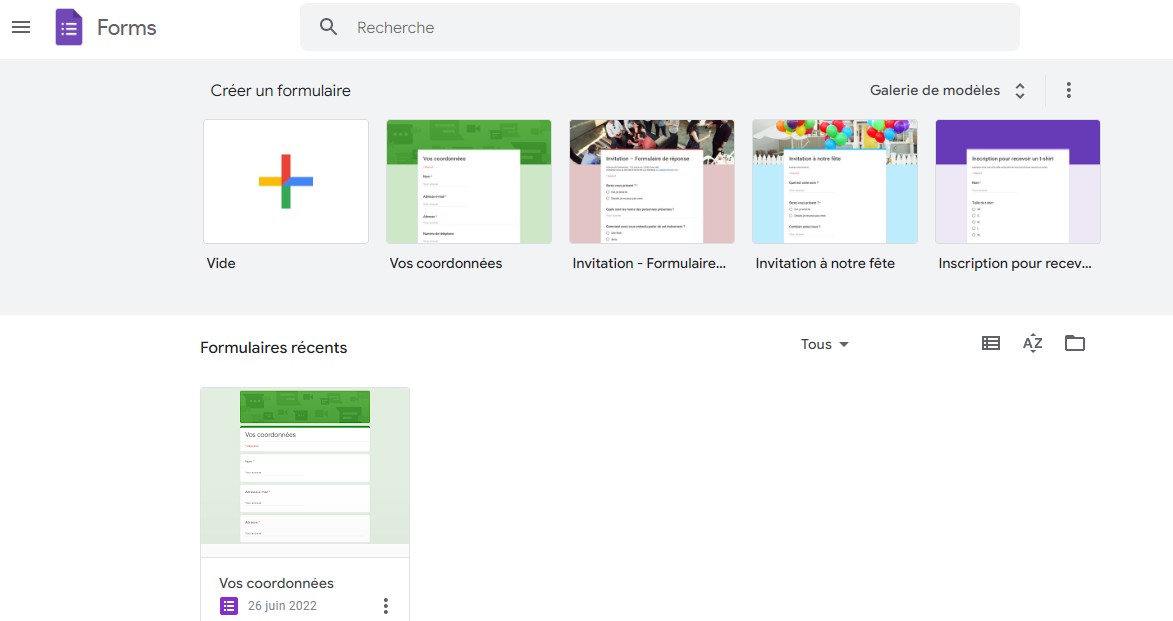
\includegraphics[width=0.95\textwidth]{D) IMAGES/for1.png}}
	\caption{Page d'Accueil Google Forms}
	\label{Org}
\end{figure}
\newpage
L’application présente trois interfaces, la première est une interface qui permet à l’utilisateur de réaliser la conception de sa fiche. \\
\begin{figure}[!h]
	\centering
	{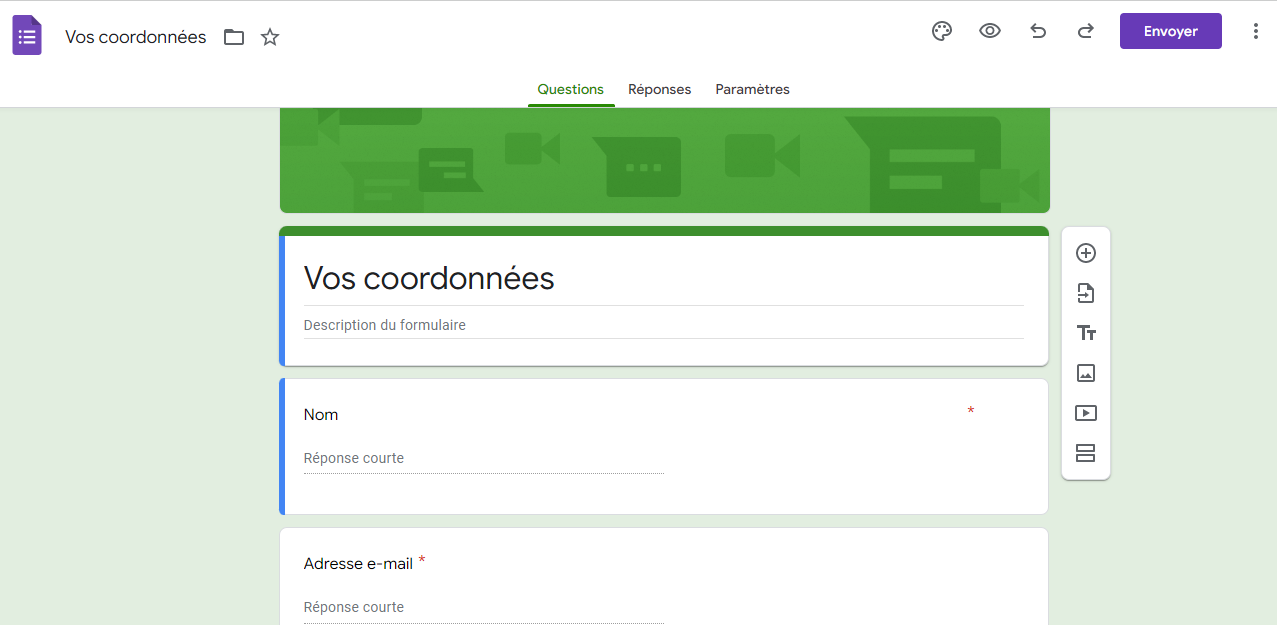
\includegraphics[width=0.95\textwidth]{D) IMAGES/for2.png}}
	\caption{Interface de conception}
	\label{Org}
\end{figure}\\
La deuxième interface est une interface d’aperçu qui permet à l’utilisateur de voir la fiche avant de faire le partage avec les autres via l’envoi du lien vers les E-mails ou bien via les réseaux sociaux (Facebook, Linkdin…).\\
\begin{figure}[!h]
	\centering
	{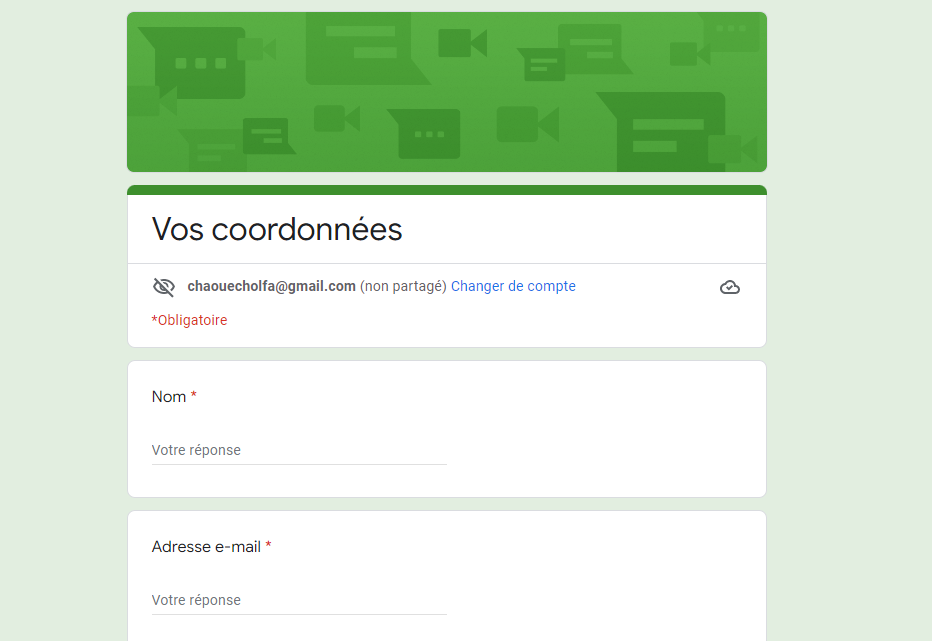
\includegraphics[width=0.95\textwidth]{D) IMAGES/forapp.png}}
	\caption{Interface d'aperçue}
	\label{Org}
\end{figure}
\\
La troisième interface est une interface de réponse qui permet au propriétaire de consulter les réponses. Les informations reçues seront décomposées en base des données.
 Une fois le formulaire d’inscription rempli en ligne, les données seront automatiquement enregistrées dans une feuille de calcul Google sous un format analysable et permettant la tabulation et la représentation graphique de données.
\begin{figure}[!h]
	\centering
	{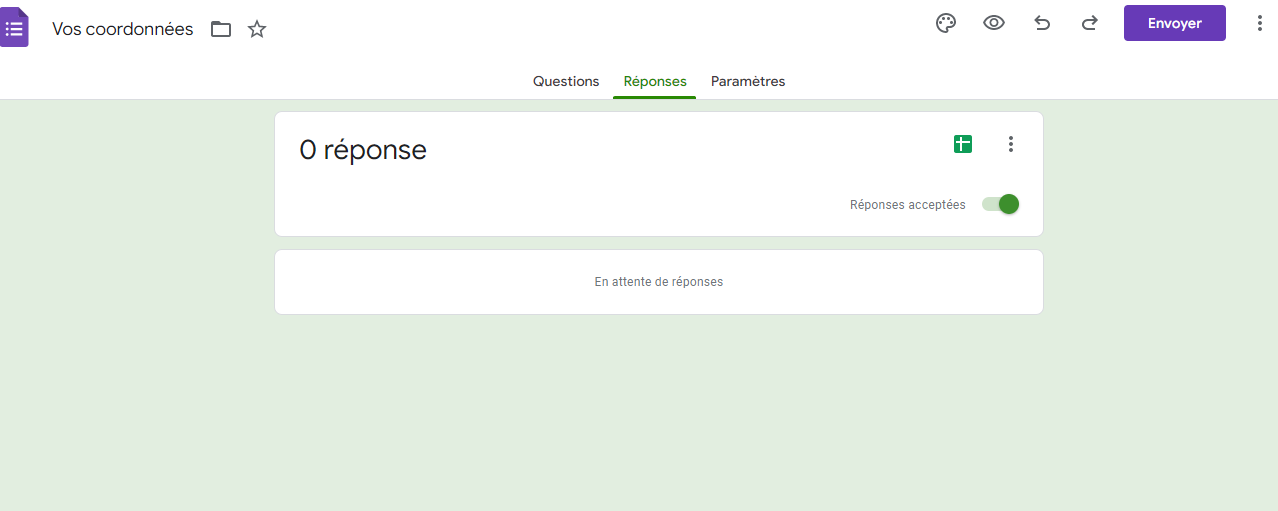
\includegraphics[width=0.95\textwidth]{D) IMAGES/for3.png}}
	\caption{Interface de réponse}
	\label{Org}
\end{figure}
\newpage
\subsection{Critique de l'existant}
Google Forms est un outil de gestion de données basé sur le cloud utilisé pour concevoir et développer des formulaires en ligne, il présente un inconvénient majeur au niveau de sécurité de données personnelles.\\
En effet, selon L’INPDP suite à son usage «Les données personnelles relatives à 13 universités, 203 établissements publics d’enseignement supérieur et 72 établissements privés sont quotidiennement violées, ce qui équivaut à 300 structures d’enseignement et à des milliers d’étudiants, dénonce-t-elle dans un communiqué publié jeudi 28 octobre 2021\footnote{\url{https://www.webmanagercenter.com/2021/10/28/474672/violation-a-grande-echelle-des-donnees\\-personnelles-dans-le-milieu-universitaire-tunisien-sinquiete-linpdp}}. Elle appelle les autorités de tutelle à intervenir pour protéger les données personnelles des étudiants et de tout le personnel travaillant dans le secteur de l’enseignement supérieur.»  
\subsection{Solution proposée}
Le CNUDST dispose d’un site web déployé moyennant le CMS WordPress qui utilise PHP comme langage de programmation et MySQL comme base de données. Les modules de gestion des formations à développer, intégreront le site web via le développement d’un nouveau thème pour assurer les inscriptions aux formations en ligne et un plugin pour gérer les formations et les inscriptions à ces formations.\\
\textbf{Présentation de Wordpress}\\
WordPress est un système de gestion de contenu (SGC) ou CMS (Content Management System) en anglais\footnote{Pour plus d’informations sur le CMS visiter le lien suivant \url{https://www.ionos.fr/digitalguide/hebergement/cms/comparatif-des-meilleurs-cms/} }. Il s’agit d’un système extensible basé sur PHP et MySQL.\\Son architecture est divisée en trois parties principales : les composants de base, les thèmes et les plugins.\\Les composants de base implémentent des fonctionnalités essentielles accessibles via des API que les plugins peuvent utiliser, les thèmes gèrent l'apparence du contenu (par exemple, la mise en page) et les plugins ajoutent des extensions à WordPress.\\
Selon les statistiques fournies par le site \url{https://w3techs.com/}, Wordpress occupe 43.3$\%$ du marché global (de tous les sites web dans le monde) et 65.3 $\%$ concernant le marché des CMS (les sites web créés avec un CMS identifiable). Il est à noter que 33.7 $\%$ des sites web ont été créés sans CMS.
\newpage
\begin{figure}[!h]
	\centering
	{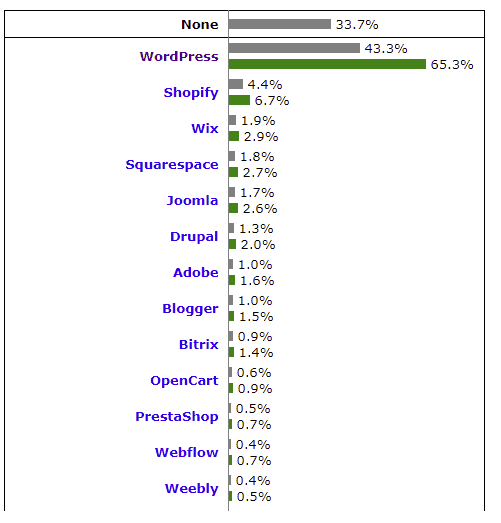
\includegraphics[width=0.75\textwidth]{D) IMAGES/cmsMarche.png}}
	\caption{Part de marché Wordpress}
	\label{CMSWordPress}
\end{figure}

\begin{table}[!h]
	\centering % used for centering table
	\begin{tabular}{ |p{7cm}|p{7cm}| } 
	
		
		\hline% inserts single horizontal line
	\textbf{Avantages} & \textbf{Inconvénients} \\
		\hline
		 Grande Communauté & Les fonctionnalités de CMS nécessitent des extensions supplémentaires\\ 
		 	\hline  
		Faibles coûts d'installation et de configuration & Les plugins ont souvent des failles de sécurité   \\ 
			\hline
		 Interface utilisateur intuitive & Stabilité et performances réduites\\
		  	\hline
		 Intégration facile des plugins & Mises à jour fréquentes de sécurité, ce qui conduit à une administration supplémentaire et parfois lourde  \\ 
	  
		\hline \hline
	
	\end{tabular}
	\begin{flushright}
		\footnotesize Source: Digital guide ionos: Comparatif de CMS 2022 .\end{flushright}
	\caption{Avantages et Inconvénients de WordPress}
\end{table}
Par mesure de sécurité, le CNUDST a choisi de développer ses propres plugins au lieu d'utiliser les plugins fournis par WordPress.\\
Notre objectif consiste donc à développer un plugin pour assurer la gestion des thèmes de formation, des formations et des inscriptions en ligne\footnote{voir la carte mentale du projet à l'annexe 1}.

\section{Choix du framework de gestion de projet}
Au cours des dernières décennies, de nouvelles méthodes sont apparues pour gérer des projets et développer des logiciels. L'idéologie agile était
généralement définie avec le manifeste agile en 2001 et est largement utilisée pour la gestion de projets logiciels. Scrum est
la méthode la plus courante au sein d'agile et est devenue l'un des outils les plus populaires dans le développement de logiciels.\\
Scrum
a une position forte dans le développement de logiciels avec ses rôles définis, son accent sur la collaboration, sa compréhension, sa visibilité, son processus efficace et son développement rapide.

L'objectif de cette section consiste à mettre l'accent sur la façon dont Scrum est appliqué. 
\subsection{Présentation de l’approche agile}
Certains chercheurs ont défini "Agile" comme une philosophie. En effet, selon\\ \cite{highsmith2001agile}"Agile implique d'être efficace et maniable. Un processus Agile est à la fois léger et suffisant. La légèreté est un moyen de rester maniable. \cite{boehm2004balancing} décrit les méthodes Agiles comme "une excroissance d'une expérience de prototypage et de développement rapide ainsi que la résurgence d'une philosophie selon laquelle la programmation est un processus artisanal plutôt qu'industriel"
La suffisance est une question de rester dans le jeu." De sa part, \cite{larman2004agile} a déclaré : « Il n'est pas possible de définir exactement les méthodes agiles, car les pratiques spécifiques varient. Cependant, des itérations limitées dans le temps avec des raffinements adaptatifs et évolutifs des plans et des objectifs".\\
Une autre manière pour décrire les méthodes Agiles consiste à énoncer les pratiques de base partagées par les différentes méthodes Agiles. Selon la définition de \cite{boehm2004balancing} qui est plus basée sur la pratique ",  en général, les méthodes agiles sont des processus très légers qui utilisent des cycles d'itération courts ; Impliquer activement les utilisateurs pour établir, hiérarchiser et vérifier les exigences ; et s'appuyer sur des connaissances tacites au sein d'une équipe plutôt que sur la documentation ".\\
Plus récemment, \cite{abbas2008historical} définit la méthode Agile comme étant "une méthode adaptative, itérative et incrémentale et orientée vers les clients.
\begin{itemize}
	\item Adaptative\\ Une méthode ouverte aux changements dans la technologie et les exigences, de plus elle répond à des retours sur des travaux antérieurs. \cite{fowler2008new} a déclaré qu'un processus adaptatif permet de contrôler l'imprévisibilité.
	\item Itératif et incrémental\\ Le logiciel est développé en plusieurs itérations, chacune de la planification à la livraison.\\
	À chaque itération, une partie du système est développée, testée et améliorée tandis qu'une nouvelle partie est en cours de développement. À chaque itération, la fonctionnalité sera améliorée.\\
	De plus, le système se développe progressivement à mesure que de nouvelles fonctionnalités sont ajoutées à chaque version.
	Après chaque itération(s), une release\footnote{Une release peut être définie comme une période de temps à l’issue de laquelle une version du livrable est proposée. Si une release possède une durée de 30 jours et que les sprints ont une durée de 15 jours, la release comportera alors 2 sprints } sera livrée au client afin d'avoir un retour d'expérience.
	\item Orientée vers les gens\\ 
	Dans une méthode Agile, les personnes sont les principaux moteurs de la réussite du projet.
	Par conséquent, le rôle du processus dans une méthode Agile est d'aider l'équipe de développement à déterminer la meilleure façon de gérer le travail.\\
	De plus, une méthode Agile met l'accent sur la communication en face à face au sein de l'équipe et avec le client qui est étroitement impliqué dans le processus de développement plutôt que sur des documents écrits."\\
	Parmi les méthodes Agiles nous citons eXtreme Programming(XP), SCRUM, Crystal Clear, Feature Driver Developpement(FDD), Lean Software Development, Dynamic System Developpement Methodology(DSDM) et Kanban.\\
	De nouvelles recherches indiquent que 52\% d'organisations utilisent la méthode SCRUM\footnote{\cite{sverrisdottir2014role}}.\\\cite{sverrisdottir2014role}, indique que"dans les méthodes agiles, les mesures de réussite d'un projet ne se limitent pas aux paramètres classiques tels que le temps, le coût et la qualité.\\ La mesure la plus importante est la fonctionnalité du produit, cette mesure est suivie par d'autres facteurs tels que la qualité, le temps/le calendrier et les aspects financiers, la taille des équipes est également importante pour le succès.\\ Il a défini trois catégories pour la taille des équipes, petite, moyenne et grande (plus de 25 personnes).\\
	Il a prouvé que plus les équipes sont petites, plus il est probable que le projet sera réussi.
	\newpage

	\begin{figure}[!h]
		\centering
		{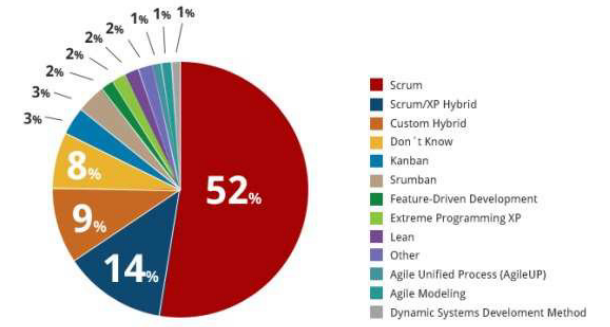
\includegraphics[width=0.85\textwidth]{D) IMAGES/agile.png}}
		\caption{Méthodes Agile}
		\label{Org}
	\end{figure}
	
\end{itemize} 

\subsection{Méthode SCRUM}
SCRUM signifie "mêlée" en français. Cette méthode aurait été définie en 1986 lorsque \cite{takeuchi1986new} ont fait des études sur des méthodes afin de développer de nouveaux produits.\\ Ils ont déclaré que "la flexibilité est l'un des facteurs les plus importants dans le processus de développement, et l'aspect le plus important est que le travail de l'équipe de développement représente une unité vers un objectif commun".\\La méthode est simple et facile à comprendre et à suivre.
Scrum met l'accent sur le contrôle du produit et une partie importante de Scrum consiste à diviser les personnes en équipes et à leur donner les moyens d'effectuer les tâches sur lesquelles elles travaillent.\\
Selon \cite{sverrisdottir2014role}, l'une des caractéristiques de Scrum est qu'une équipe Scrum est autocontrôlée, les gens sont encouragés à proposer de nouvelles idées, cela conduit à la transparence dans la prise de décision et à plus de liberté dans le processus de développement.\\La méthode est suivie d'un examen continu pendant toute la durée du développement, dans le but d'adapter les produits et les procédures de travail à l'environnement en constante évolution \footnote{\cite{sutherland2012scrum}}.\\Les connaissances sont considérées comme fondées sur l'expérience et toutes les décisions sont censées être fondées sur la connaissance.\\
Une équipe Scrum se compose de trois rôles qui sont: le Product Owner(PO), le SCRUM Master(SM) et les membres de l'Equipe.\\ Les processus de la méthode SCRUM sont: le User Story, le Product Backlog, le Sprint, le Sprint Backlog, le Burn Down Chart et le sprint meeting review. \\La méthode Scrum est illustrée graphiquement dans la figure suivante:
\begin{figure}[!h]
	\centering
	{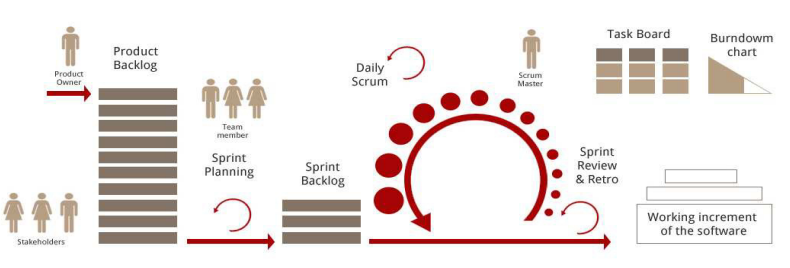
\includegraphics[width=0.95\textwidth]{D) IMAGES/scrum.png}}
	\caption{Cadre de Méthode SCRUM}
	\label{Org}
\end{figure}

\begin{enumerate}
	\item \underline{\textbf{Rôles}}
	
	\begin{itemize}
		\item \textbf{Product Owner} (Directeur du produit)\\
		Le rôle PO est l'un des rôles le plus important dans Scrum et souvent le plus difficile. Il est responsable du financement du projet pendant son cycle de vie et celui qui met le focus sur les exigences et les objectifs du projet. Il définit les spécifications fonctionnelles et établit la liste de priorités. Un PO est une seule personne, pas un groupe de personnes. Il est le représentant de toutes les parties prenantes du projet même le client. La tâche la plus importante du Product Owner est de prendre une décision sur ce qui ne doit pas être priorisé, et
		prendre les conséquences de cette décision. Il est impératif qu'il rejette les nouvelles exigences qui ne sont pas nécessaires, en
		collaboration avec les parties prenantes et l'équipe, au lieu d'ajouter de nouvelles exigences inutiles au Poduct Backlog.
		\item \textbf{SCRUM Master}\\
		La responsabilité de SM est d'assurer que le processus de la méthode SCRUM est appliqué, de plus il supervise la communication au sein de l'équipe et aide l'équipe à se concentrer sur les objectifs du projet.
		\item \textbf{Equipe}\\
		Elle est composée des développeurs, des testeurs, d'architectes et de tout 	autre métier nécessaire à la réalisation de projet.
	\end{itemize}
	\item \underline{\textbf{Processus}}
	
	\begin{itemize}
		\item \textbf{User Story}\\
		Récit utilisateur, il s'agit d'une demande fonctionnelle écrite de façon à mettre en avant les exigences hiérarchisées de l'utilisateur.\\Le product Owner s'engage d'écrire le user story d'une manière précise concernant une seule fonctionnalité. Une fois rédigée, elle va s'ajouter aux autres récits du produit et ensemble forme ce qu'on appelle le "Product backlog".
		\item \textbf{ Le Product Backlog}\\Une sorte de carnet des commandes pour le produit, le product backlog permettre de présenter ce qu'il faut faire pour réaliser les besoins de l'utilisateur et délivrer le User Story. Le Product Backlog va constamment évoluer pour refléter les nouveaux besoins. Une fois d'accord sur le Product Backlog, l'étape suivante consiste à se lancer dans la réalisation de projet ce dernier va se découper en plusieurs itérations nommées sprints dans le jargon de SCRUM.
		\item \textbf{Sprint}\\
		Un Sprint commence par une réunion de planificationn dénommée le \textbf{Sprint planning meeting}, chaque sprint dure de 2 à 4 semaines. Il y aura trois phases pendant le sprint : la phase de développement puis la phase de contrôle et la phase de livraison.\\
		L'ensemble de livraison de Sprints cumulés se nomme le \textbf{Sprint Backlog}.\\
		Durant le sprint il y a des mêlées c'est-à-dire des SCRUM qui vont être organisés chaque jour, ce sont des réunions quotidiennes d'un quart d'heure souvent effectuées au début de la journée. Elles permettent à l'équipe de mesurer l'avancement du projet et de s'assurer de la qualité de délivrable et de respect de délai.\\
		Pendant chaque réunion le SCRUM master tient d'un \textbf{Burn Down chart} pour marquer l'évolution du projet. Chaque membre de l'équipe doit pouvoir exprimer trois choses rapidement:
		\begin{itemize}
			\item Ce que vous avez fait la veille et les problèmes rencontrés.
			\item Ce que vous allez faire aujourd'hui.
			\item Les problèmes qui vous bloquent.
		\end{itemize}  
		L'objectif consiste à identifier et à communiquer les éventuels problèmes sans les résoudre pendant cette séance qui ne dépasse pas les 15 minutes.\\
		A la fin de la réunion, le SRUM Master a mis à jour le Burn Down Chart et déléguer les problèmes identifiés pendant le meeting aux membres de l'équipe.\\
		A la fin de Sprint, c'est-à-dire en général après deux semaines un autre meeting sera organisé, \textbf{le sprint meeting review}, au cours dequel la solution sera présentée au client sous forme de démonstration et d'avoir son retour, des éventuelles améliorations sont suggérées et les problèmes rencontrés seront ajoutés au Product Backlog et priorisés ensuite dans des Sprints. 
		
		
	\end{itemize}
	
\end{enumerate}


\textbf{Conclusion}\\
Tout au long de ce chapitre, nous avons présenté, en premier lieu, l'entreprise d'accueil. En second lieu, nous avons identifié l'existant tout en montrant sa critique et nous avons envisagé par la suite la solution proposée. Enfin, nous avons mis le focus sur la méthodologie utilisée.  